\chapter{Hardwareanalyse}  
\label{ch:Hardware}
Diese Projektarbeit baut auf mehreren Vorgängerprojekten auf. Bei der Übergabe wurden einige Mängel bezüglich der Konstruktion festgestellt. Deshalb wird in diesem Kapitel eine umfangreiche Hardwareanalyse durchgeführt.
Der Demonstrator besteht aktuell aus einem Airhockeytisch, einer Kamera und der Mechanik des Roboters, der den Roboterspieler verkörpert. Diese Mechanik besteht aus zwei Linearachsen, die eine Bewegung des “Pushers” in einer Ebene ermöglichen. Angesteuert werden die beiden Motoren mittels eines Arduinos. Das Arduino wird mit einer seriellen Schnittstelle erreicht. Bei den Motoren handelt es sich um Schrittmotoren, die mit einem Riemen einen Schlitten auf einer Führung entlang der Linearachsen bewegen. Um mehr Stabilität und Dynamik zu erreichen, wurde eine H-Anordnung für den Aufbau der Führungswellen gewählt.  

\section{Aufbau}
\label{sect:Aufbau}

Für eine bessere Übersicht sind in den nachfolgenden Abbildungen \ref{HW_Aufbau} und \ref{HW_Kamerahalterung} die einzelnen Komponenten eingetragen, welche im Folgenden genauer betrachtet werden.\\
Die Funktionsweise des hier bereits realisierten Aufbaus besteht aus zwei Elektromotoren (1), die jeweils ein Zahnrad (4) antreiben. Über einen fest gespannten Zahnriemen und mehrere Umlenkrollen kann der Schlitten inklusive des Pushers (7) in neun mögliche Richtungen entlang der Führungswellen (2, 6) bewegt werden. Diese sind von den jeweiligen Laufrichtungen der zwei Motoren abhängig. 
Zur Aufnahme des Spielfelds für ein späteres Spiel gegen den trainierten Agenten ist oberhalb des Mittelpunkts eine Kamera (9) auf einer Querstrebe befestigt.\\
\clearpage
\begin{figure}
\includegraphics[width=1\textwidth]{images/HW_Aufbau}
 \caption{(1) Motor und Motorgehäuse;
(2)	Führungswelle (Längsrichtung);
(3)	Schlitten auf der Führungswelle (Längsrichtung);
(4)	Zahnrad;
(5)	Hintere Halterung der Führungswelle (Längsrichtung);
(6)	Führungswelle (Querrichtung);
(7)	Aufnahmeschlitten für den Pusher des Trainierten Agenten
}
\label{HW_Aufbau}
\end{figure}

\begin{figure}
\includegraphics[width=1\textwidth]{images/HW_Kamerahalterung}
\caption[width=0.5\textwidth]{(8) Befestigung der Querstrebe für die Kamerahalterung; (9) Kamera}
\label{HW_Kamerahalterung}
\end{figure}
\clearpage

\section{Komponentenaustausch}
\label{sect:Komponentenaustausch}
Die Komponenten des Hardwareaufbaus werden für eine bessere Übersicht in drei Gruppen eingeteilt. Die erste Gruppe "Bewegung des Roboters" beinhaltet alle Komponenten, die für das dynamische Bewegen des Pushers (7) beteiligt sind (vgl. Abbildung \ref{HW_Aufbau}). Die Gruppe zwei "Bilderfassung" enthält die Kamera inklusive dem Halter und dem dazugehörigen Aufbau (vgl. Abbildung \ref{HW_Kamerahalterung}). Mit der letzten Gruppe "Original Airhockeytisch" ist der Originalaufbau des Airhockeytisches, so wie dieser gekauft wurde, gemeint.\\

\underline{Bewegung des Roboters}:
\begin{figure} [h]
\begin{minipage}[t]{\textwidth}
\vspace{0pt}
Die Bewegungen des Pushers (7) sind nur dann ideal, wenn der Zahnriemen fest gespannt wird. Aufgrund eines fehlenden Endanschlags am hinteren Halter (5) der Führungswelle in Längsrichtung (2) und des zu festen Spannen des Zahnriemens wirkte eine zu große Kraft F am Motorengehäuse (1), sodass dieses leicht nach vorne geneigt war (Winkel $\alpha$). Begünstigt durch die Aussparungen des HHN Logos und diese zuvor beschriebene Kraft F brach das Gehäuse (1) an einigen Stellen auseinander. In der Abbildung \ref{HW_Motorgehaeuse} sind beide Effekte zu erkennen.\\
\end{minipage}
\end{figure}

\begin{figure} [h]

\begin{minipage}[t]{0.6\textwidth}
\vspace{0pt}
\includegraphics[width=\textwidth]{images/HW_Motorgehaeuse}
\caption{Neigung des Motorgehäuses um Winkel $\alpha$ aufgrund der Kraft F und der daraus resultierende Riss am Motorengehäuse ist rot umrandet.\\}
\label{HW_Motorgehaeuse}
\end{minipage}
\end{figure}

\clearpage




\begin{figure} [h]

\begin{minipage}[t]{0.45\textwidth}
\vspace{0pt}
Zur Lösung dieses Problems wurde zunächst das Motorgehäuse (1) ohne Aussparungen und mit verstärkter Wanddicke 3D gedruckt. Auch neu gedruckt wurden die hinteren Halterungen der Führungswelle in Längsrichtung (5), sodass diese Welle (2) nun mit einem Keil in der Halterung festgeklemmt werden kann und somit der Kraft F entgegenwirkt. In der Abbildung \ref{HW_HKeil} ist diese hintere Halterung, durch den die Welle mithilfe des Keils (rot umkreist) fixiert wird, dargestellt.
\end{minipage}
\hspace{0.1\textwidth}
\begin{minipage}[t]{0.4\textwidth}
\vspace{0pt}
\includegraphics[width=\textwidth]{images/HW_Hintere_Halterung_Keil}
 \caption{Hintere Halterung der Führungswelle in Längsrichtung mit rot gekennzeichnetem Keil zur Verklemmung dieser Welle.}
 \label{HW_HKeil}
\end{minipage}
\end{figure}


\begin{figure} [h]

\begin{minipage}[t]{0.45\textwidth}
\vspace{0pt}
Im Zuge der gesamten Stabilisierung des Zahnriemenantriebs wurden die zwei Antriebszahnräder aus dem 3D Drucker durch industriell hergestellte Aluminiumzahnräder ersetzt. Des Weiteren wurden auch die 3D gedruckten Umlenkrollen für die Spannvorrichtung durch industriell Gefertigte ersetzt. In der nachfolgenden Abbildung \ref{HW_Umlenkrolle} ist diese Spannvorrichtung aus dem 3D Drucker rot umkreist dargestellt.
\end{minipage}
\hspace{0.1\textwidth}
\begin{minipage}[t]{0.4\textwidth}
\vspace{0pt}
\includegraphics[width=\textwidth]{images/HW_Umlenkrolle}
\caption{Umlenkrolle für die Spannvorrichtung aus dem 3D Drucker ist rot markiert.}
 \label{HW_Umlenkrolle}
\end{minipage}
\end{figure}

\begin{figure} [h]

\begin{minipage}[t]{0.45\textwidth}
\vspace{0pt}
Eine weitere Auffälligkeit war die Verdrehung der Führungswellen in Querrichtung (6). In Abbildung \ref{HW_VQuer} ist dies deutlich erkennbar, denn die Führungswellen sollten parallel zu den blauen Linien auf dem Spieltisch stehen. Das ist aber nicht der Fall. \\
Diese Verdrehung hatte zur Folge, dass das Ansteuern von einem bestimmten Punkt mit dem Pusher (7) fast nicht möglich war, da z. B. bei einer reinen Querbewegung auch ein kleiner Anteil an Längsbewegung als Störung dazu kam.
\end{minipage}
\hspace{0.1\textwidth}
\begin{minipage}[t]{0.4\textwidth}
\vspace{0pt}
\includegraphics[width=\textwidth]{images/HW_VerdrehungQuerstrebe}
 \caption{Verdrehung der Führungswellen in Querrichtung}
\label{HW_VQuer}
\end{minipage}
\end{figure}



\begin{figure} [h]

\begin{minipage}[t]{0.45\textwidth}
\vspace{0pt}
Gelöst wurde dieses Problem durch eine Vergrößerung der Einfassungen der Querstreben in den Schlitten (3) auf der Führungswelle in Längsrichtung. Abbildung \ref{HW_HVQuer} zeigt den Vergleich zwischen der neuen verbauten Version und der alten, darunter auf dem Tisch liegenden Version. Der Unterschied ist eine Erweiterung der Einfassungen der Querstreben.\\
Bei anschließenden Tests konnten keine Richtungsabweichungen mehr festgestellt werden.
\end{minipage}
\hspace{0.1\textwidth}
\begin{minipage}[t]{0.4\textwidth}
\vspace{0pt}
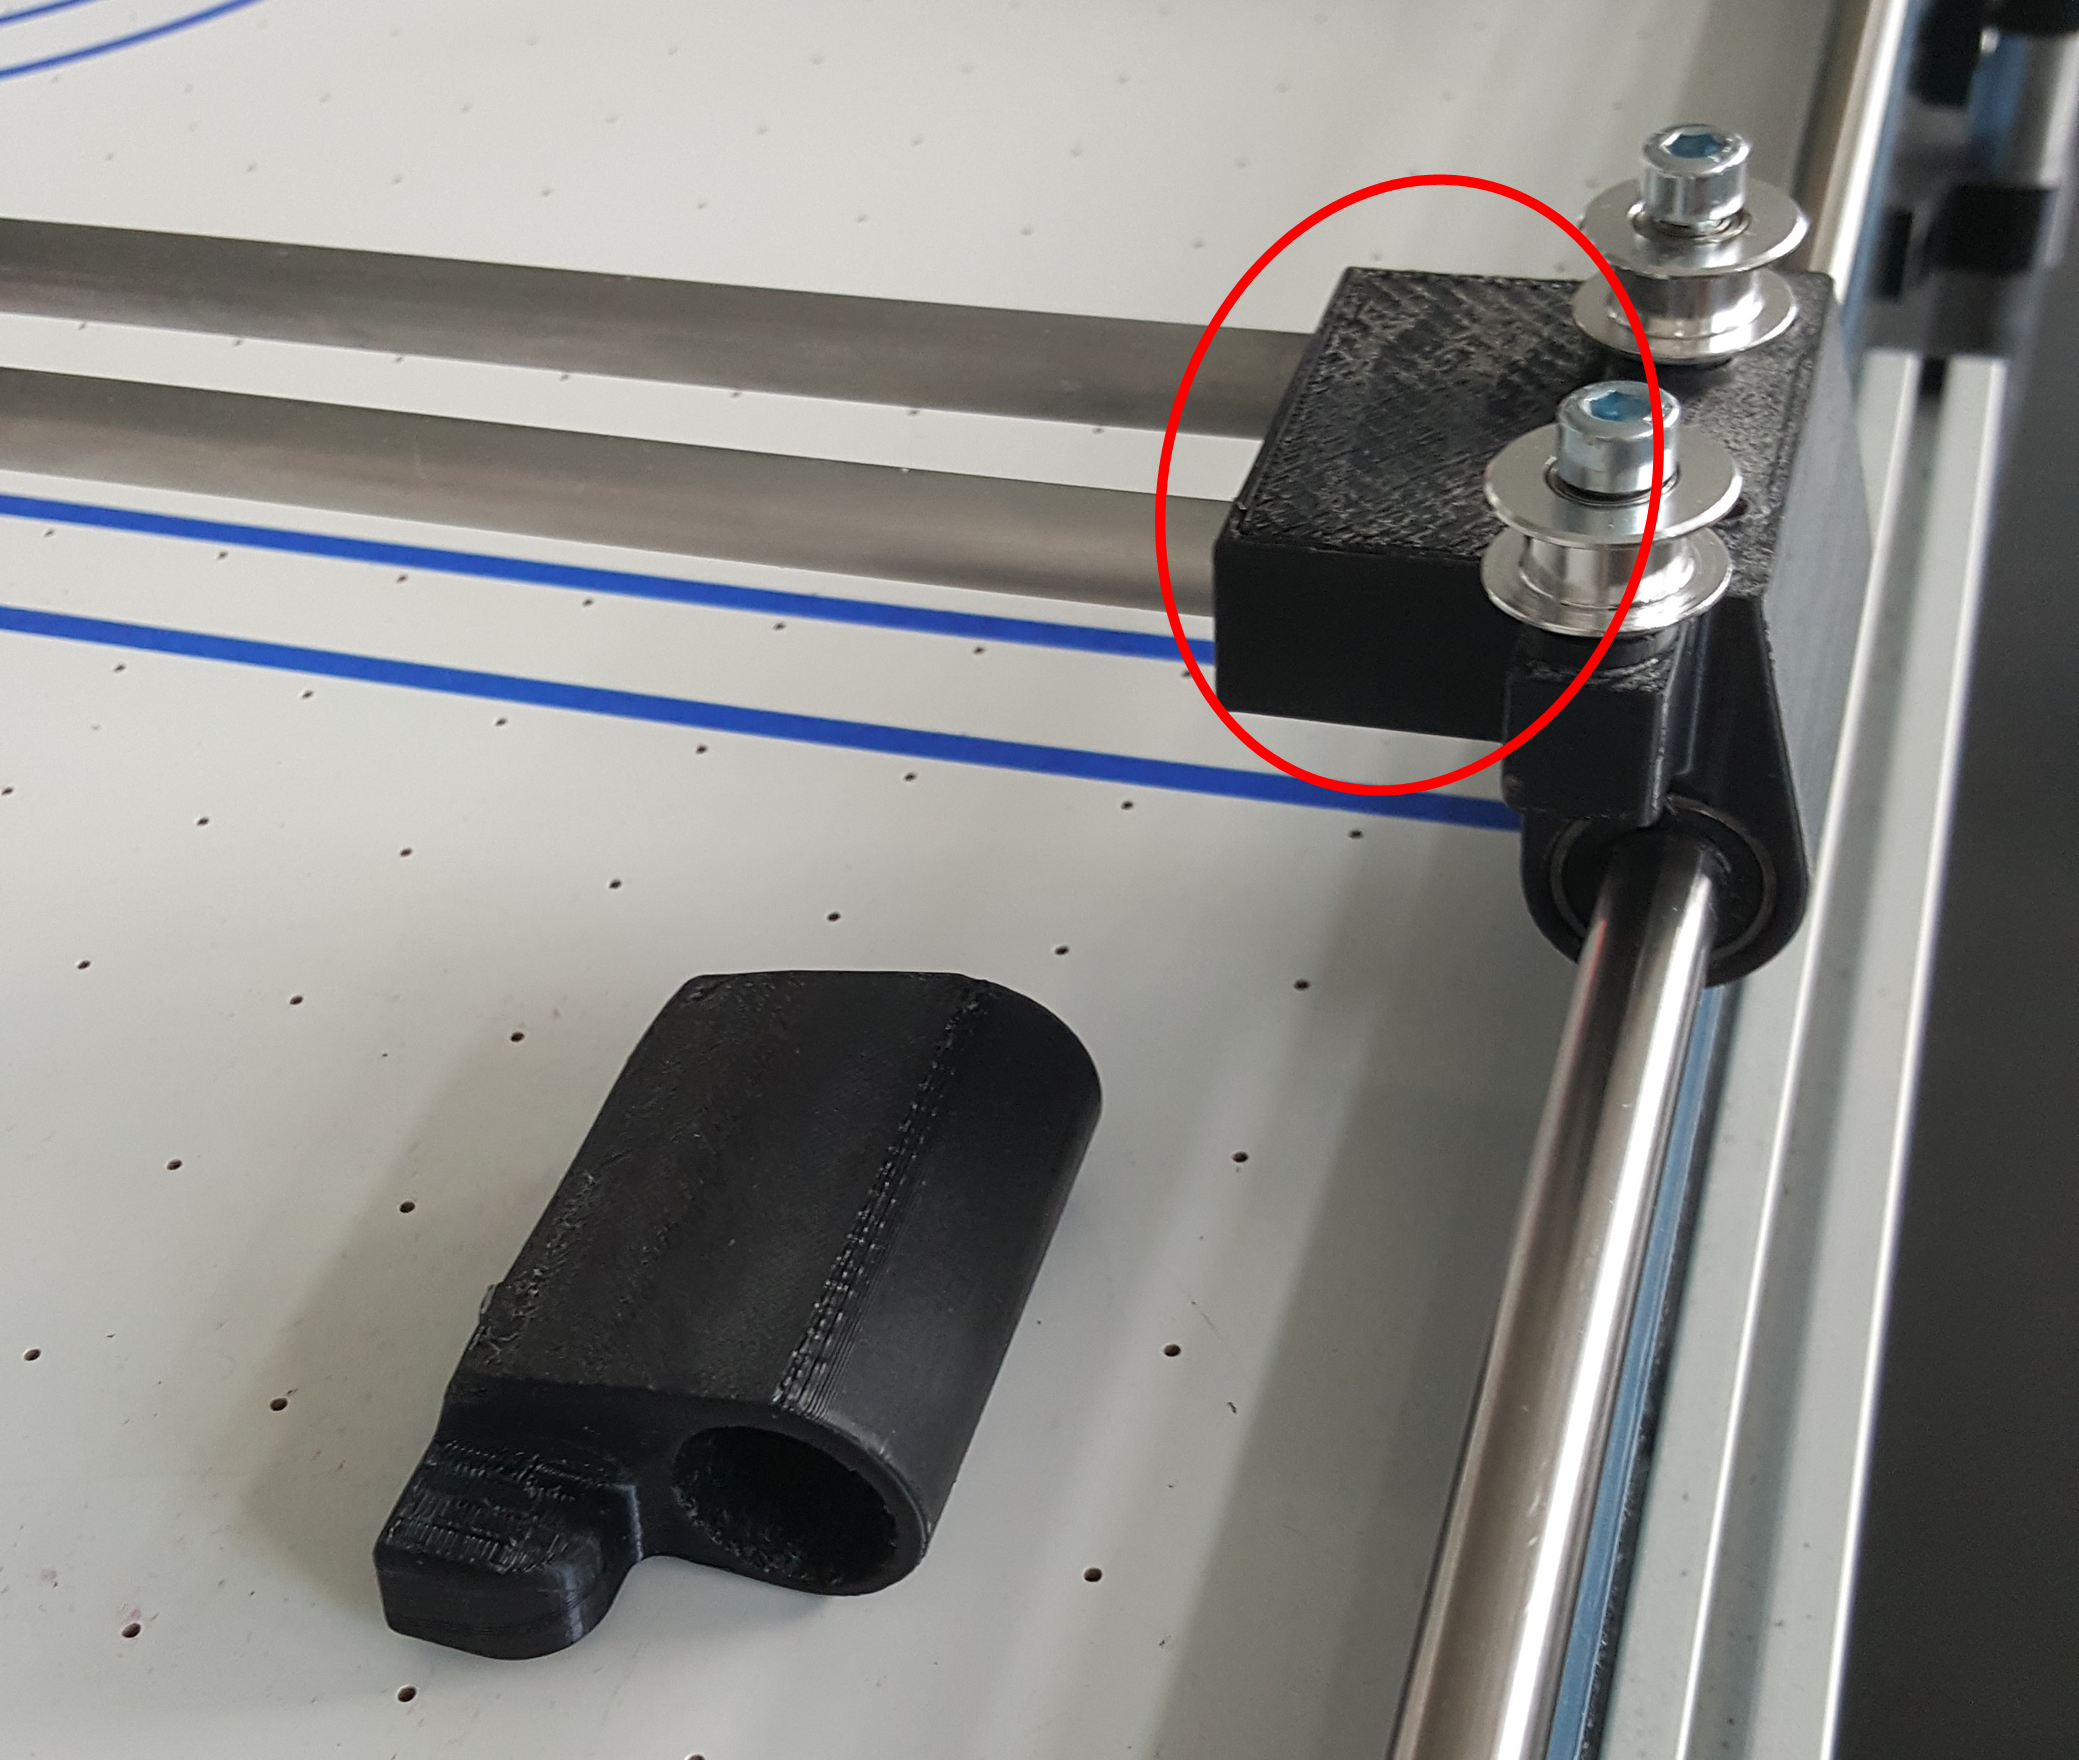
\includegraphics[width=\textwidth]{images/HW_Halterung_FQ}
 \caption{Vergleich der Schlitten (3): Neue Version ist verbaut, die alte Version liegt auf dem Tisch darunter (Orientierung: Der alte Schlitten ist um $90^\circ$  Richtung Tischplatte gedreht. }
\label{HW_HVQuer}
\end{minipage}
\end{figure}
\clearpage 




\underline{Bilderfassung}:
\begin{figure} [h]

\begin{minipage}[t]{\textwidth}
\vspace{0pt}
    Eine weitere Komponente, die verbessert werden musste, war die Befestigung der Querstrebe für die Kamerahalterung (8). Bei der bisherigen Lösung wurde diese obere Stange, auf der die Kamera (9) mittig fest fixiert ist, links und rechts in die Bögen aus dem 3D Drucker (8) lose eingesteckt. Um eine Verdrehung der Kamera (9) bzw. der Stange zu verhindern, wurde diese mit Madenschrauben an den Plastikverbindungsstücken fixiert. Durch zu festes Zudrehen der Madenschrauben sind beide Halterungen jedoch gebrochen.\\
\end{minipage}
\end{figure}

\begin{figure} [h]

\begin{minipage}[t]{\textwidth}
\vspace{0pt}
\includegraphics[width=\textwidth]{images/HW_Kamera_gebrochen}
\caption{Riss am Befestigungsbogen für die Querstrebe der Kamerahalterung.\\}
\label{HW_Kamera_gebrochen}

\end{minipage}
\end{figure}
 
Da der Schwerpunkt der Kamera (9) inklusive der Halterung leicht versetzt zum Schwerpunkt der oberen Stange liegt, wirkt dieses Moment gegen die Fixierungen mit den Madenschrauben. Dies hatte zur Folge, dass sich diese Stange und die darauf fixierte Kamera langsam drehten. Damit veränderte sich das Sichtfeld der Kamera kontinuierlich, bis es zum Schluss nicht mehr den gesamten Spieltisch umfasste.\\
Um dieses Problem zu umgehen, wurde ein anderer Ansatz zur Befestigung der Querstrebe gewählt. Die neu konstruierten 90° Bögen (8) besitzen Aussparungen in Längsrichtung, sodass das Ende des Bogens leicht zusammengedrückt werden kann. Die Querstrebe wird nun mithilfe von Rohrschellen darin fest verklemmt. Der Vorteil an einer Fixierung mit einer Rohrschelle gegenüber einer mit Madenschraube ist, dass die Kraft nun nicht konzentriert auf eine kleine Stelle wirkt, sondern auf den kompletten Umfang verteilt wird.\\

\clearpage

\underline{Original Airhockeytisch}:\\
\\Die größte Herausforderung bei der Optimierung des Hardwareaufbaus bestand darin, dass der Pusher (7) in der Nähe der Tischkante, insbesondere der Torlinie, oftmals ins Stocken gerät oder sogar ganz stecken bleibt. Eine genauere Betrachtung der Spielplatte zeigte, dass diese in der Spieltischmitte leicht absinkt und an den Banden wieder ansteigt. Es ist möglich, den Pusher wenige Millimeter in der Höhe zu verstellen, indem entweder Distanzscheiben in die innen liegende Verschraubung hinzugefügt oder entfernt werden.\\ Da diese Höhenverschiebung erst gegen Ende des Projekts durchgeführt wurde, kam es bereits beim Testen zuvor zu Rissbildungen am Pusher (7). In der Abbildung \ref{HW_Pusher} können die Risse links und rechts jeweils an der Aufnahme der Führungswellen (6) erkannt werden. \\
\begin{figure} [h]

\begin{minipage}[t]{0.6\textwidth}
\vspace{0pt}
\includegraphics[width=\textwidth]{images/HW_Pusher}
\caption{Risse am Pusherschlitten antlang der Einfassung der Führungswellen in Querrichtung.\\}
\label{HW_Pusher}

\end{minipage}
\end{figure}
\clearpage

Wenn jedoch der Abstand zwischen Tisch und Pusher zu groß ist, kann es passieren, dass der Puck dazwischen eingeklemmt wird. Leider ist es mit dem aktuellen Aufbau nicht möglich, beide Probleme gleichzeitig zu lösen.\\
\\Des Weiteren reduziert sich die Geschwindigkeit des Pucks beim Überqueren der Aufkleber auf dem Tisch und durch Verschmutzungen an der Oberfläche. Dadurch kommt es zu unerwarteten Schwankungen, was die Übertragung von Simulationsergebnissen auf den realen Aufbau nachteilig beeinflusst.\\





